\section{Ejercicio 5}
En el presente ejercicio se analiza la ejecución del siguiente código.

\lstinputlisting[language={[Motorola68k]Assembler}]{code/ej5.asm} 

\subsection{Status Register inicializado en \$0300}
Se imponen las siguientes condiciones iniciales a los registros.
$$ a = \$00000000000000 $$
$$ sr = \$0300 $$

Dentro de estas condiciones se destaca que el valor inicial del status register considera ambos bits de escala (S1, S0) en cero, por lo que no se produce escalamiento en el valor del acumulador. 

En la tabla~\ref{tab:ej5_instructions_a} se observa como se desarrolla la ejecución del programa en cuestión.

\begin{table}[H]
\centering
\begin{tabular}{|c|c|c|}
\hline
\textbf{Instrucción} & \textbf{Cambios}                                                           & \textbf{Comentarios}                                                                                                   \\ \hline
-                  & \begin{tabular}[c]{@{}c@{}}a = \$00000000000000\\ sr = \$0300\end{tabular} & Carga inicial de valores.                                                                                              \\ \hline
move \#\$400000,x0     & x0 = \$400000                                                              & \begin{tabular}[c]{@{}c@{}}Carga el valor inmediato en x0.\\ No hay cambios en el sr.\end{tabular}                     \\ \hline
add x0,a             & \begin{tabular}[c]{@{}c@{}}a = \$00400000000000\\ sr = \$0300\end{tabular} & \begin{tabular}[c]{@{}c@{}}Suma el valor de x0 en a.\\ a = 0,5.\\ El acumulador estaba inicializado en 0.\end{tabular} \\ \hline
add x0,a             & \begin{tabular}[c]{@{}c@{}}a = \$00800000000000\\ sr = \$0320\end{tabular} & \begin{tabular}[c]{@{}c@{}}Suma el valor de x0 en a.\\ a = 1.\\ Se activa el bit Extension (E=1).\end{tabular}         \\ \hline
\end{tabular}
\caption{Paso a paso de las instrucciones ejecutadas con sr=\$0300}
\label{tab:ej5_instructions_a}
\end{table}

La tabla~\ref{tab:ej5_results_a} refleja el estado final de los registros.

\begin{table}[H]
\centering
\begin{tabular}{|c|c|c|}
\hline
\textbf{Registro} & \textbf{Valor inicial} & \textbf{Valor final} \\ \hline
a                 & \$00000000000000       & \$00800000000000     \\ \hline
sr                & \$0300                 & \$0320               \\ \hline
\end{tabular}
\caption{Estado inicial y final de los registros con sr=\$0300}
\label{tab:ej5_results_a}
\end{table}

Se observa que luego de la ejecución del segundo \textit{add}, el acumulador toma el valor a = \$00800000000000. Esto surge de que se suma dos veces el valor 0,5, contenido en x0. De esta forma, el valor final del acumulador a es 1. Luego, el bit de extensión (E) del CCR se activa, indicando que se está usando la parte entera del acumulador. Esto sucede dado que en un número de punto fijo de 24 bits no es posible representar la unidad.


\begin{figure}[H]
    \centering
    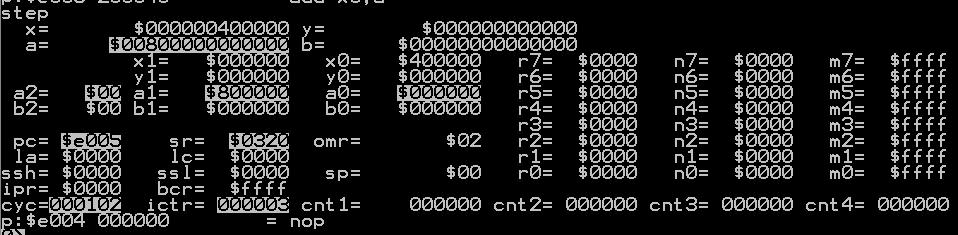
\includegraphics[width=\textwidth]{figs/ej5/ej5_3_a.png}
    \caption{Estado final de los registros con sr=\$0300 (simulación).}
    \label{fig:ej5_simregs_a}
\end{figure}

En la figura~\ref{fig:ej5_simregs_a} se observa el resultado de la simulación.


\subsection{Status Register inicializado en \$0700}
Se repite el análisis anterior, pero esta vez con las siguientes condiciones iniciales:

$$ a = \$00000000000000 $$
$$ sr = \$0700 $$

Esta vez se comienza con el bit de escalamiento S0 activo. Esta condición implica que se produce un shift aritmético hacia la izquierda de los acumuladores. De esta forma, se desplaza el punto fraccionario un lugar hacia la izquierda. Esto cambia la forma en la que el DSP computa los bits \textit{Unnormalized} y \textit{Extension} (U y E, respectivamente) del CCR.
\\
En la tablas~\ref{tab:ej5_instructions_b} y \ref{tab:ej5_results_b} se muestra el paso a paso en la ejecución de las instrucciones y los resultados, respectivamente.

\begin{table}[H]
\centering
\begin{tabular}{|c|c|c|}
\hline
\textbf{Instrucción} & \textbf{Cambios}                                                           & \textbf{Comentarios}                                                                                                      \\ \hline
-                  & \begin{tabular}[c]{@{}c@{}}a = \$00000000000000\\ sr = \$0700\end{tabular} & Carga inicial de valores.                                                                                                 \\ \hline
move \#\$400000,x0     & x0 = \$400000                                                              & \begin{tabular}[c]{@{}c@{}}Carga el valor inmediato en x0.\\ No hay cambios en el sr.\end{tabular}                        \\ \hline
add x0,a             & \begin{tabular}[c]{@{}c@{}}a = \$00400000000000\\ sr = \$0710\end{tabular} & \begin{tabular}[c]{@{}c@{}}Suma el valor de x0 en a.\\ a=0,5.\\ Se activa el bit Unnormalized del ccr (U=1).\end{tabular} \\ \hline
add x0,a             & \begin{tabular}[c]{@{}c@{}}a = \$00800000000000\\ sr = \$0700\end{tabular} & \begin{tabular}[c]{@{}c@{}}Suma el valor de x0 en a.\\ Se desactiva el bit Unnormalized del ccr (U=0).\end{tabular}       \\ \hline
\end{tabular}
\caption{Paso a paso de las instrucciones ejecutadas con sr=\$0700}
\label{tab:ej5_instructions_b}
\end{table}

\begin{table}[H]
\centering
\begin{tabular}{|c|c|c|}
\hline
\textbf{Registro} & \textbf{Valor inicial} & \textbf{Valor final} \\ \hline
a                 & \$00000000000000       & \$00800000000000     \\ \hline
sr                & \$0700                 & \$0700               \\ \hline
\end{tabular}
\caption{Estado inicial y final de los registros con sr=\$0700}
\label{tab:ej5_results_b}
\end{table}

De las tablas anteriores se concluye que el resultado en el acumulador a no cambió respecto del caso expuesto en la tabla~\ref{tab:ej5_results_a}. En contraposición, se aprecia que el comportamiento del CCR durante la ejecución es distinto que el de la tabla~\ref{tab:ej5_instructions_a}. Como se advirtió anteriormente, esto se debe al cambio en las condiciones de escalamiento impuestas por el nuevo valor inicial del status register, y en cómo estas afectan al cálculo de ciertos bits del mismo.

En este caso, al ejecutar el primer \textit{add}, se carga el valor \$00400000000000 en el acumulador a. Dado que ahora se trabaja con el punto fraccionario desplazado una posición hacia la izquierda, no se cumple la condición de normalización, activando el bit correspondiente en el CCR que indica que el acumulador no se encuentra normalizado. Al sumar nuevamente el valor de x0, pasa a cumplirse la condición de normalización y el bit U cambia su valor a 0.

Otra diferencia respecto al caso anterior es que luego de ejecutadas las instrucciones, no se activa el bit de extensión del CCR. Nuevamente, esto se debe al desplazamiento hacia la izquierda del punto fraccionario. En este caso, esta modificación resulta en que el valor final del acumulador sea 0,5 en lugar de 1, lo cual implica que no se está haciendo uso de la parte entera del mismo.


\begin{figure}[H]
    \centering
    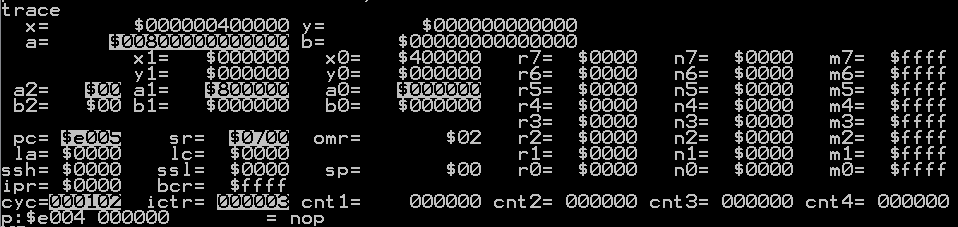
\includegraphics[width=\textwidth]{figs/ej5/ej5_3_b.png}
    \caption{Estado final de los registros con sr=\$0700 (simulación).}
    \label{fig:ej5_simregs_b}
\end{figure}

La figura~\ref{fig:ej5_simregs_b} muestra el resultado de la simulación realizada.
